\section{黄金分割法}

%-----------------------------------------------------------
% 1. 黄金分割法
%-----------------------------------------------------------
\begin{frame}
    \frametitle{黄金分割法の歴史}
    黄金分割法の原理に基づく探索手順は、1953年にKieferの論文「Sequential Minimax Search for a Maximum」の中で提案されました。
    この論文の主題は観測回数が固定されたときフィボナッチ数を用いた探索法でしたが、
    黄金分割法も同時に紹介されました。
\end{frame}

% このファイルは自動生成されました
% 親ファイル(tex_soturonhappyoルート)から \input して使用することを想定しています

% フレーム1: フィボナッチ法（補足1）
\begin{frame}
  \frametitle{フィボナッチ法による最適探索}
  \begin{columns}
    \begin{column}{0.45\textwidth}
      \small
      \textbf{補足：} Kiefer氏は観測回数が固定された場合、フィボナッチ数を用いた探索法を提示しました。
      
      \vspace{0.5em}
      \begin{itemize}
        \item 観測回数が\textbf{事前に決定}されている
        \item フィボナッチ数により最悪ケースを最適化
        \item 関数値が小さい側に拡大
        \item 赤点：新規評価点
      \end{itemize}
      
      \vspace{0.5em}
      \textbf{目的関数:} $f(x) = (x-2)^2 + 0.5\sin(3x)$
    \end{column}
    \begin{column}{0.55\textwidth}
      \centering
      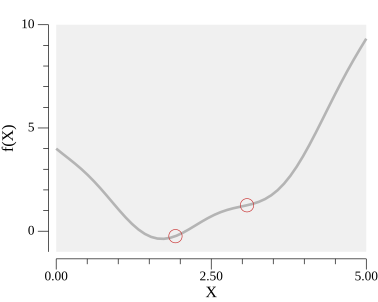
\includegraphics[width=\textwidth]{material/kiefer/output/fibonacci_fixed_obs.png}
    \end{column}
  \end{columns}
\end{frame}

% フレーム2: 黄金比を用いた方法（補足2）
\begin{frame}
  \frametitle{黄金比を用いたアルゴリズム}
  \begin{columns}
    \begin{column}{0.45\textwidth}
      \small
      \textbf{補足：} これとは別に、黄金比を用いて常に同じアルゴリズムで区間を縮小する手順が提示されました。
      
      \vspace{0.5em}
      \begin{itemize}
        \item 黄金比 $\phi = \frac{\sqrt{5}-1}{2} \approx 0.618$
        \item \textbf{同じアルゴリズム}を繰り返す
        \item 観測回数は事前に決めない
        \item 関数が単峰性を保つ限り有効
      \end{itemize}
      
      \vspace{0.5em}
      これが一般に\textbf{黄金分割法}と呼ばれます。
    \end{column}
    \begin{column}{0.55\textwidth}
      \centering
      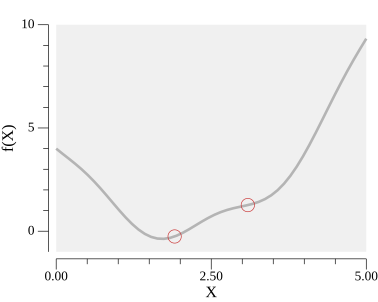
\includegraphics[width=\textwidth]{material/kiefer/output/golden_ratio_method.png}
    \end{column}
  \end{columns}
\end{frame}

% フレーム3: 黄金分割法の実用性（補足3）
\begin{frame}
  \frametitle{黄金分割法の実用性}
  \begin{columns}
    \begin{column}{0.45\textwidth}
      \small
      \textbf{補足：} 黄金分割法は厳密には最適な手順ではありませんが、観測回数を事前に決めない場合に特に有用です。
      
      \vspace{0.5em}
      \begin{itemize}
        \item 各段階で区間は最悪でも $0.618$ 倍に縮小する
        \item 実装が簡単で安定している
        \item 収束性が良好
        \item 観測回数を任意に変更可能
      \end{itemize}
      
      \vspace{0.5em}
      \textbf{利点:} 実用性と安定性のバランスが優れている
    \end{column}
    \begin{column}{0.55\textwidth}
      \centering
      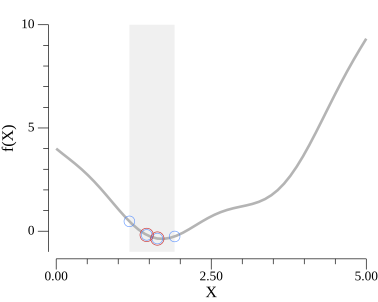
\includegraphics[width=\textwidth]{material/kiefer/output/golden_section_no_fixed_obs.png}
    \end{column}
  \end{columns}
\end{frame}





% このファイルは自動生成されました。
% 親ファイル(tex_soturonhappyoルート)から \input して使用することを想定しています。
\begin{frame}{黄金分割法の収束プロセス}
  \begin{columns}
    \begin{column}{0.4\textwidth}
      \begin{itemize}
        \item \textbf{グレー領域}: 現在の探索区間
        \item \textcolor{red}{\textbf{赤丸}}: 今回の評価点
        \item \textcolor{blue}{\textbf{青丸}}: 既存の評価点
      \end{itemize}
      \vspace{1em}
      範囲が狭まるにつれ、範囲外の点は探索対象から除外（消去）されます。
    \end{column}
    \begin{column}{0.6\textwidth}
      \centering
      \only<1>{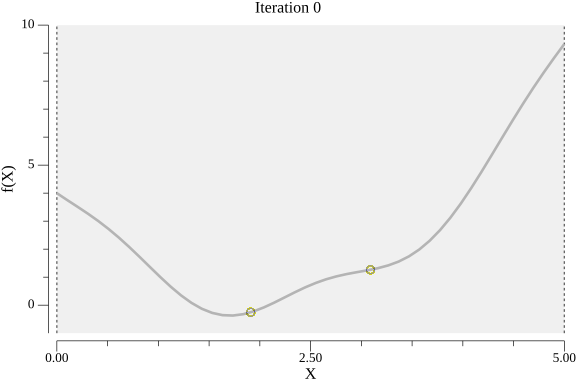
\includegraphics[width=\textwidth]{material/golden/output/golden_00.png}}
      \only<2>{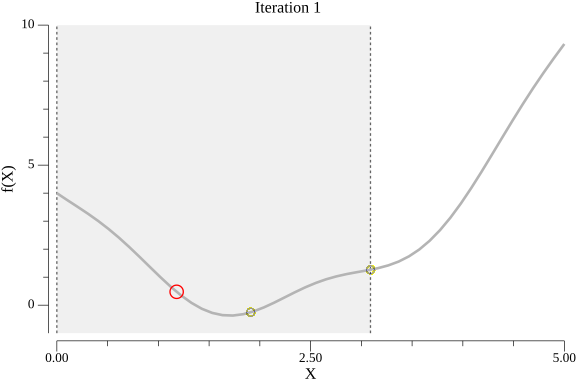
\includegraphics[width=\textwidth]{material/golden/output/golden_01.png}}
      \only<3>{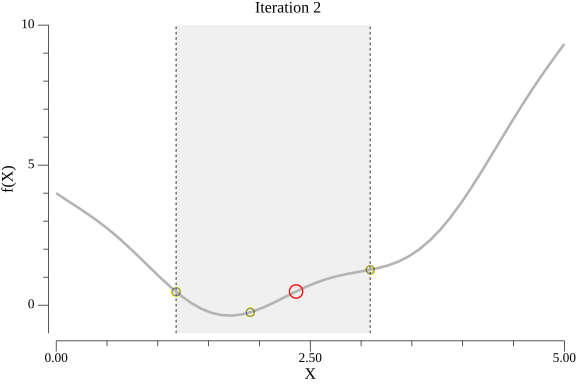
\includegraphics[width=\textwidth]{material/golden/output/golden_02.png}}
      \only<4>{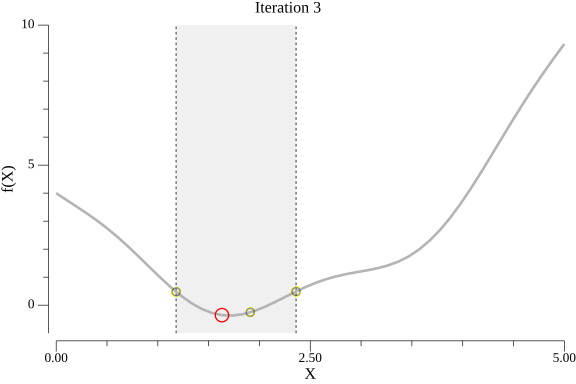
\includegraphics[width=\textwidth]{material/golden/output/golden_03.png}}
      \only<5>{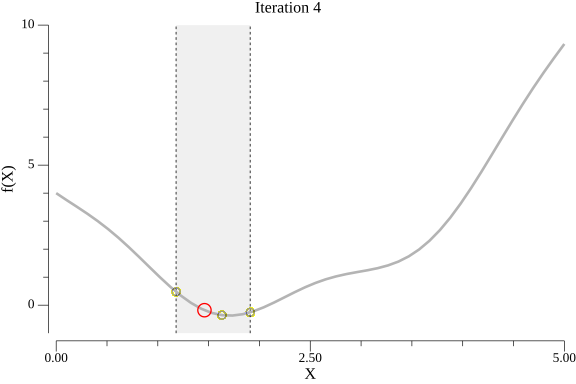
\includegraphics[width=\textwidth]{material/golden/output/golden_04.png}}
      \only<6>{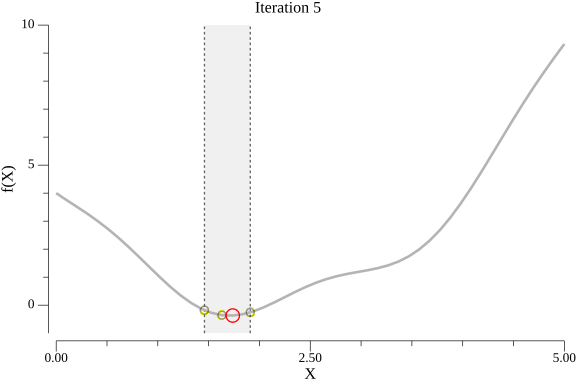
\includegraphics[width=\textwidth]{material/golden/output/golden_05.png}}
      \only<7>{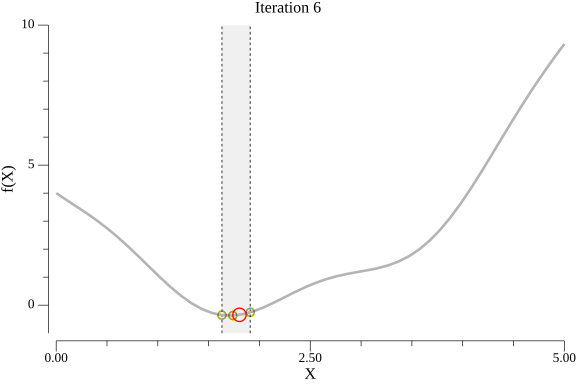
\includegraphics[width=\textwidth]{material/golden/output/golden_06.png}}
      \only<8>{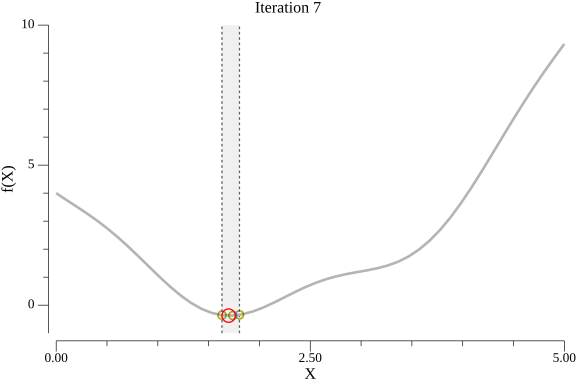
\includegraphics[width=\textwidth]{material/golden/output/golden_07.png}}
      \only<9>{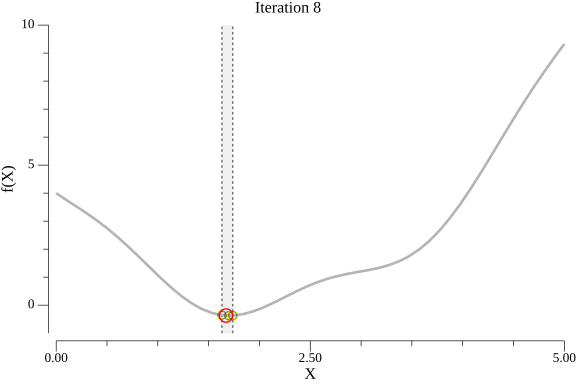
\includegraphics[width=\textwidth]{material/golden/output/golden_08.png}}
      \only<10>{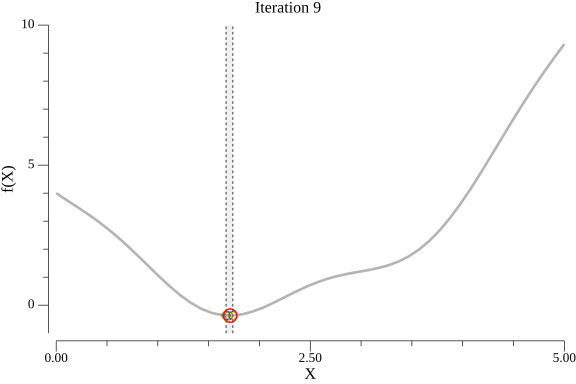
\includegraphics[width=\textwidth]{material/golden/output/golden_09.png}}
      \only<11>{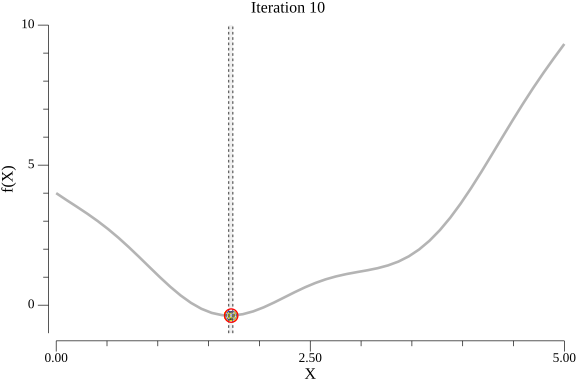
\includegraphics[width=\textwidth]{material/golden/output/golden_10.png}}
      \only<12>{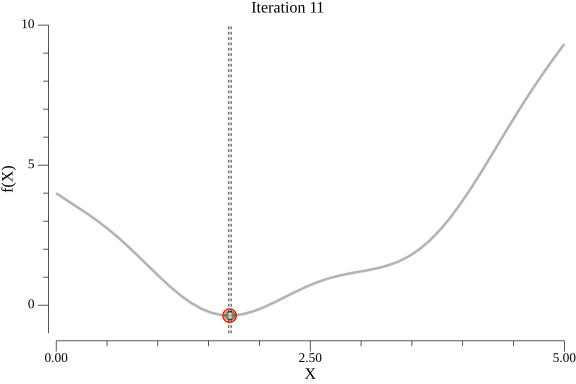
\includegraphics[width=\textwidth]{material/golden/output/golden_11.png}}
      \only<13>{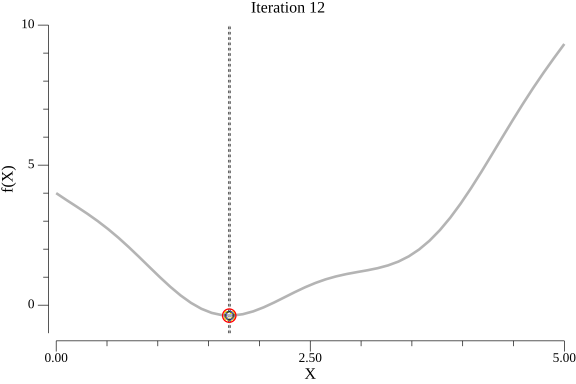
\includegraphics[width=\textwidth]{material/golden/output/golden_12.png}}
      \only<14>{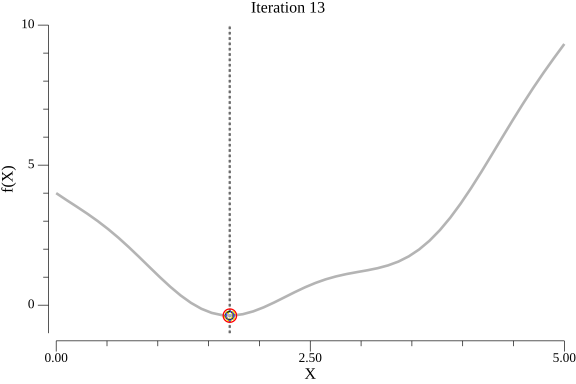
\includegraphics[width=\textwidth]{material/golden/output/golden_13.png}}
      \only<15>{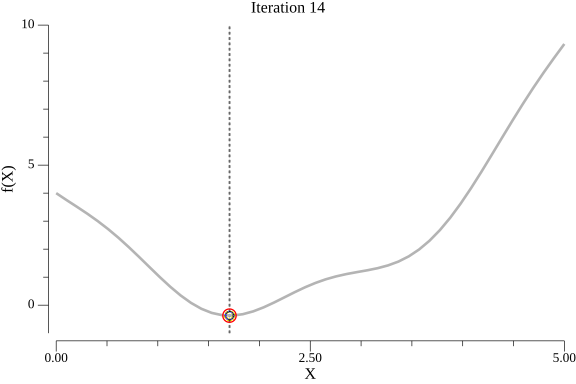
\includegraphics[width=\textwidth]{material/golden/output/golden_14.png}}
      \only<16>{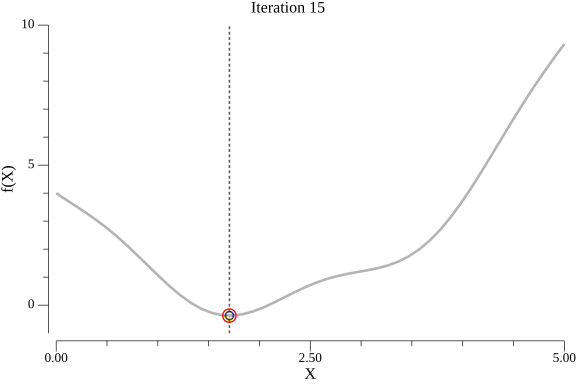
\includegraphics[width=\textwidth]{material/golden/output/golden_15.png}}
    \end{column}
  \end{columns}
\end{frame}


\begin{frame}
\frametitle{黄金分割法の収束性}
\section*{1. 新しい点の位置関係の定義}
極小を囲う3点 $a < b < c$ について、比率 $W$ と $Z$ を定義します。
\begin{itemize}
    \item $W = \frac{b-a}{c-a}$
    \item $1-W = \frac{c-b}{c-a}$
\end{itemize}

\centering
\vspace{0.2cm}
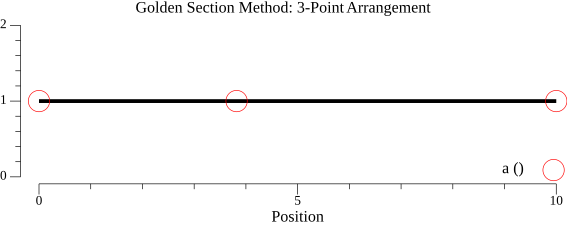
\includegraphics[width=0.7\textwidth]{material/convergence/output/diagram1_points.png}
\end{frame}

\begin{frame}
\frametitle{黄金分割比の導出（2）}
\section*{2. 最悪ケースの縮小率最適化}
新しい点 $x$ の位置を、最悪ケースの縮小率を最適化するために決定します：
\begin{itemize}
    \item 条件: $ W+Z = 1-W $
    \item 導出: $ Z = 1 - 2W $
\end{itemize}

\centering
\vspace{0.2cm}
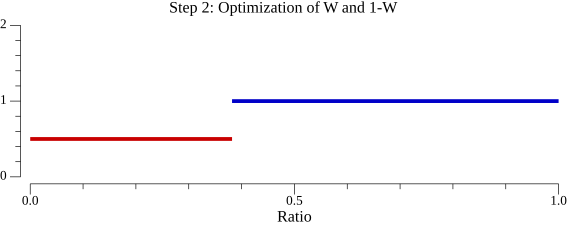
\includegraphics[width=0.7\textwidth]{material/convergence/output/diagram2_optimization.png}
\end{frame}

\begin{frame}
\frametitle{黄金分割比の導出（3）}
\section*{3. スケール相似性}
新しい区間でも同じ比率を保つという相似性の原理：
\begin{itemize}
    \item 相似条件: $ \frac{Z}{1-W} = W $
    \item 新区間と元区間の比率が常に等しい
\end{itemize}

\centering
\vspace{0.2cm}
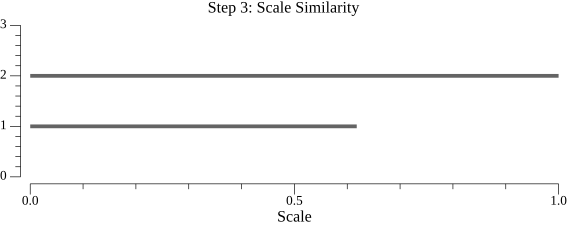
\includegraphics[width=0.7\textwidth]{material/convergence/output/diagram3_similarity.png}
\end{frame}

\begin{frame}
\frametitle{黄金分割比の導出（4）・収束性}
\section*{4. 黄金分割比と収束率}
比率条件より、以下の方程式を得ます：
\begin{itemize}
    \item 二次方程式: $ W^2 - 3W + 1 = 0 $
    \item 解: $ W = \frac{3 - \sqrt{5}}{2} \approx 0.38197 $
    \item 黄金比: $ \phi = \frac{\sqrt{5}-1}{2} \approx 0.618 $
    \item 収束率: 各ステップで区間は $\phi$ 倍に縮小（1次収束）
\end{itemize}

\centering
\vspace{0.2cm}
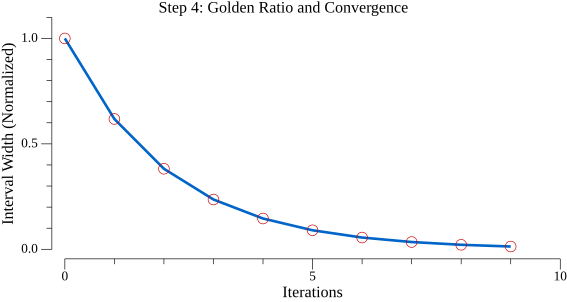
\includegraphics[width=0.7\textwidth]{material/convergence/output/diagram4_convergence.png}
\end{frame}
